%%%%%%%%%%%%%%%%%%%%%%%%%%%%%%%%%%%%%%%%%
% Beamer Presentation
% LaTeX Template
% Version 1.0 (10/11/12)
%
% This template has been downloaded from:
% http://www.LaTeXTemplates.com
%
% License:
% CC BY-NC-SA 3.0 (http://creativecommons.org/licenses/by-nc-sa/3.0/)
%
%%%%%%%%%%%%%%%%%%%%%%%%%%%%%%%%%%%%%%%%%

%----------------------------------------------------------------------------------------
%	PACKAGES AND THEMES
%----------------------------------------------------------------------------------------

\documentclass{beamer}

\mode<presentation> {

% The Beamer class comes with a number of default slide themes
% which change the colors and layouts of slides. Below this is a list
% of all the themes, uncomment each in turn to see what they look like.

%\usetheme{default}
%\usetheme{AnnArbor}
%\usetheme{Antibes}
%\usetheme{Bergen}
%\usetheme{Berkeley}
%\usetheme{Berlin}
%\usetheme{Boadilla}
%\usetheme{CambridgeUS}
%\usetheme{Copenhagen}
%\usetheme{Darmstadt}
%\usetheme{Dresden}
%\usetheme{Frankfurt}
%\usetheme{Goettingen}
%\usetheme{Hannover}
%\usetheme{Ilmenau}
%\usetheme{JuanLesPins}
%\usetheme{Luebeck}
\usetheme{Madrid}
%\usetheme{Malmoe}
%\usetheme{Marburg}
%\usetheme{Montpellier}
%\usetheme{PaloAlto}
%\usetheme{Pittsburgh}
%\usetheme{Rochester}
%\usetheme{Singapore}
%\usetheme{Szeged}
%\usetheme{Warsaw}

\useoutertheme{miniframes} % Alternatively: miniframes, infolines, split
\useinnertheme{circles}

% As well as themes, the Beamer class has a number of color themes
% for any slide theme. Uncomment each of these in turn to see how it
% changes the colors of your current slide theme.

%\usecolortheme{albatross}
%\usecolortheme{beaver}
%\usecolortheme{beetle}
%\usecolortheme{crane}
%\usecolortheme{dolphin}
%\usecolortheme{dove}
%\usecolortheme{fly}
%\usecolortheme{lily}
%\usecolortheme{orchid}
%\usecolortheme{rose}
%\usecolortheme{seagull}
%\usecolortheme{seahorse}
%\usecolortheme{whale}
%\usecolortheme{wolverine}

%%% Try color %%%
% \definecolor{gold}{RGB}{212, 175, 55}
% \definecolor{mahidolBlue}{RGB}{37,57,136}
% \definecolor{mahidolYellow}{RGB}{165,128,46}
% \definecolor{orangeSCMU}{RGB}{255,140,0}
% \definecolor{olivegreen}{RGB}{34,139,34}

% \setbeamercolor{palette primary}{bg=mahidolBlue,fg=orangeSCMU!40}
% \setbeamercolor{palette secondary}{bg=mahidolBlue,fg=white}
% \setbeamercolor{palette tertiary}{bg=mahidolBlue,fg=white}
% \setbeamercolor{palette quaternary}{bg=mahidolBlue,fg=white}
% \setbeamercolor{structure}{fg=mahidolBlue} % itemize, enumerate, etc
% \setbeamercolor{section in toc}{fg=mahidolBlue} % TOC sections
% \setbeamercolor{subsection in head/foot}{bg=orangeSCMU!90,fg=white}
%%% End color %%%

%\setbeamertemplate{footline} % To remove the footer line in all slides uncomment this line
%\setbeamertemplate{footline}[page number] % To replace the footer line in all slides with a simple slide count uncomment this line

%\setbeamertemplate{navigation symbols}{} % To remove the navigation symbols from the bottom of all slides uncomment this line
}

\usepackage{tikz}
\usepackage{transparent}
\usepackage{graphicx} % Allows including images
\usepackage{booktabs} % Allows the use of \toprule, \midrule and \bottomrule in tables
\usepackage{dirtytalk}

%----------------------------------------------------------------------------------------
%	TITLE PAGE
%----------------------------------------------------------------------------------------

\title[Outlier Detection for DC]{Outlier Detection for Data Certification} % The short title appears at the bottom of every slide, the full title is only on the title page

\author{Patomporn Payoungkhamdee} % Your name
\institute[MU] % Your institution as it will appear on the bottom of every slide, may be shorthand to save space
{
Mahidol University \\ % Your institution for the title page
\medskip
\textit{patomporn.pay@gmail.com} % Your email address
}
\date{2 August 2019} % Date, can be changed to a custom date

\begin{document}

\begin{frame}
\titlepage % Print the title page as the first slide
\end{frame}

\begin{frame}
\frametitle{Overview} % Table of contents slide, comment this block out to remove it
\tableofcontents % Throughout your presentation, if you choose to use \section{} and \subsection{} commands, these will automatically be printed on this slide as an overview of your presentation
\end{frame}

%----------------------------------------------------------------------------------------
%	PRESENTATION SLIDES
%----------------------------------------------------------------------------------------

%------------------------------------------------
\section{Background} % Sections can be created in order to organize your presentation into discrete blocks, all sections and subsections are automatically printed in the table of contents as an overview of the talk
%------------------------------------------------

\subsection{} % A subsection can be created just before a set of slides with a common theme to further break down your presentation into chunks

\begin{frame}
\frametitle{Data Quality Monitoring (DQM)}

\begin{figure}
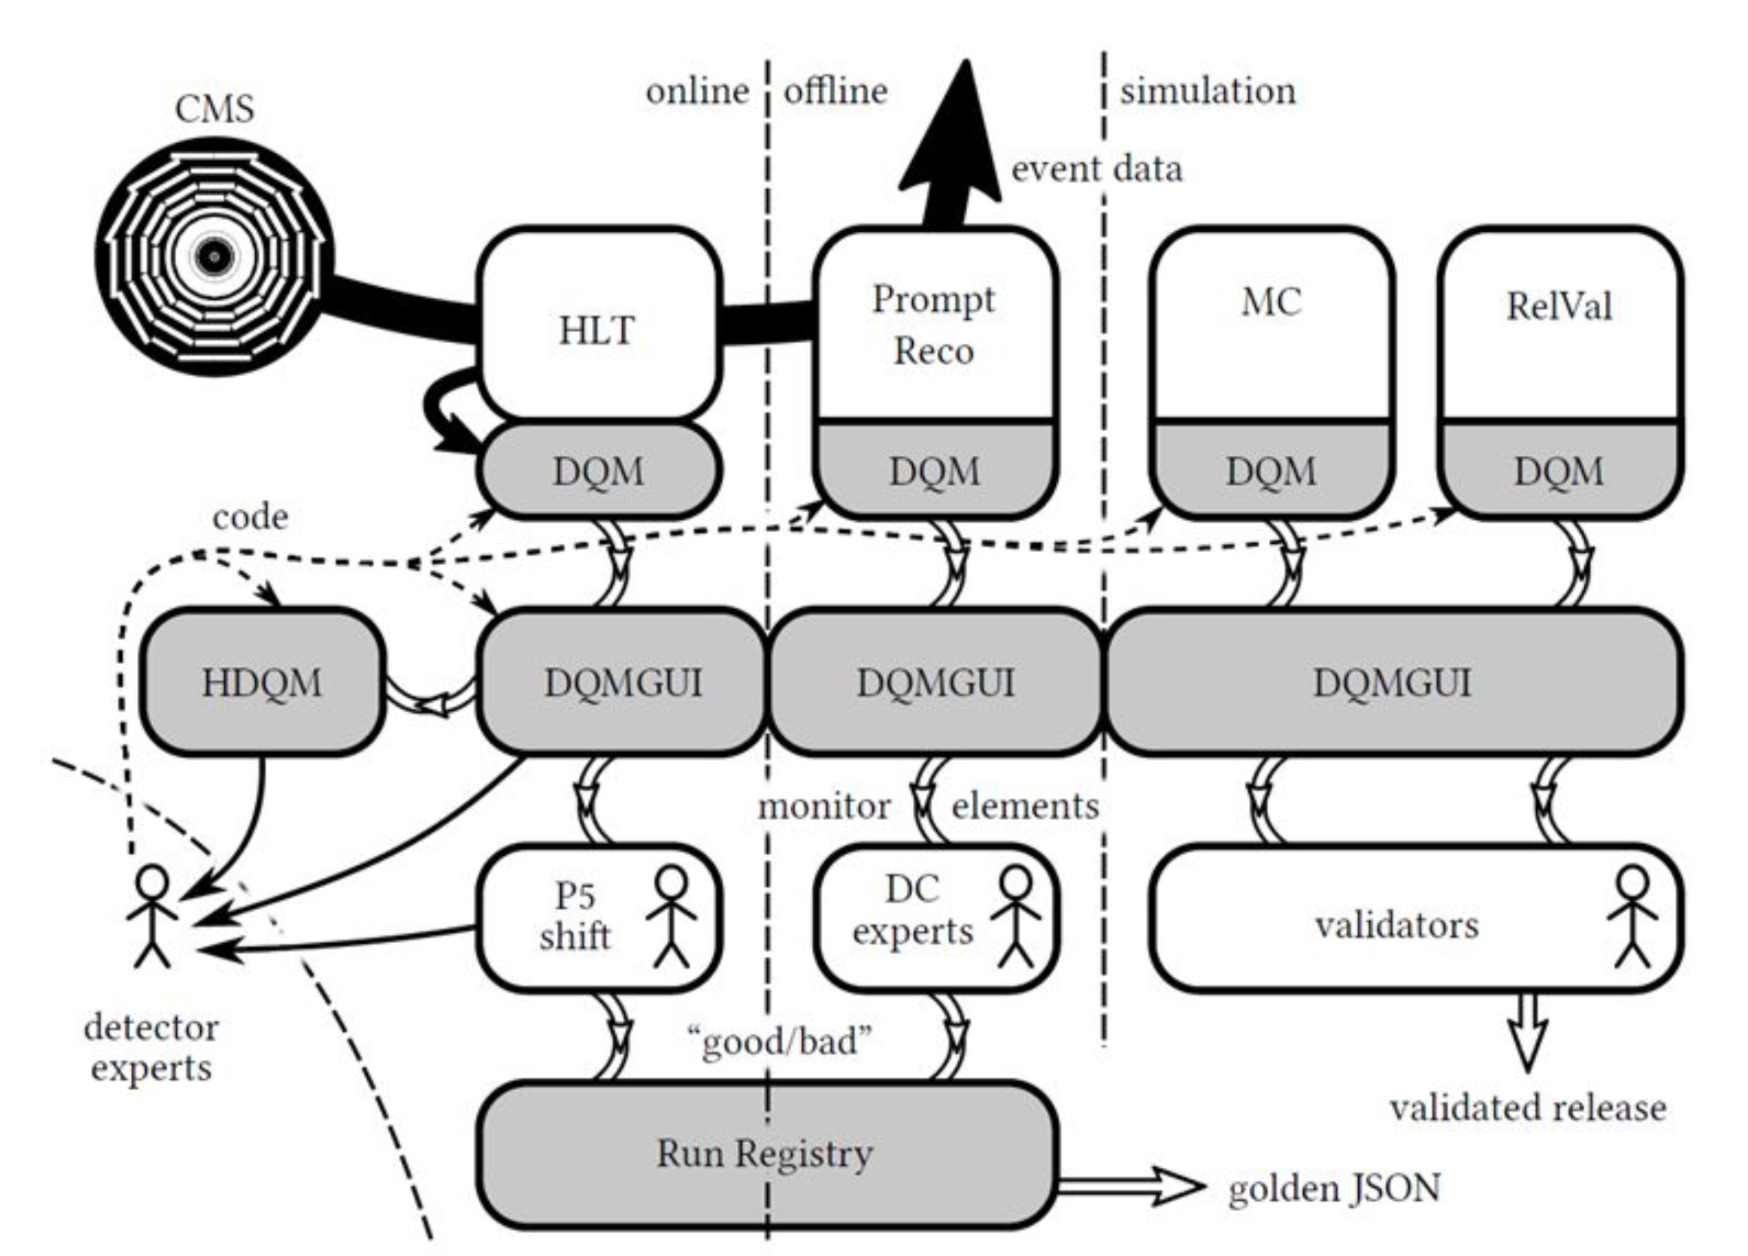
\includegraphics[height=0.7\textheight, width=0.7\textwidth]{images/dqm_flow}
\caption{Tools and Processes of DQM, retrieved from M. Stankevičius }
\end{figure}

\end{frame}

%------------------------------------------------

\begin{frame}
\frametitle{Data granularity in CMS (Offline)}
\begin{itemize}
    \item Reconstruct physics quantity 48 Hours after collision 
    \item Offline shifters and detector experts check the dozens of distribution histograms to define goodness of data
    \item Certification is made on Run and Lumisection levels
    \item Lumisection(LS) is taken around 23 seconds for one interval
    \item Briefly criteria for bad LS
    \begin{enumerate}
        \item Runs tagged as bad by human (whole run)
        \item DCS bits (LS levels)
        \item Shifter mark some range of LSs from other cases
    \end{enumerate}
    \item Golden JSON are the rest of them (Good LS)
\end{itemize}
\vspace{0.4in}\tiny [1] M. Stankevičius, Data Quality Monitoring: Offline
\end{frame}

%------------------------------------------------
\section{Objective} % Sections can be created in order to organize your presentation into discrete blocks, all sections and subsections are automatically printed in the table of contents as an overview of the talk
%------------------------------------------------
\subsection{}

\begin{frame}
\frametitle{Objective}
\begin{itemize}
    \item \textbf{Certify data quality in lumisection granularity}
    \item Reduce manual work of the shifter
    \item Standardize data certification criteria
\end{itemize}
\end{frame}

%------------------------------------------------

\begin{frame}
\frametitle{Expectation}
\begin{figure}
    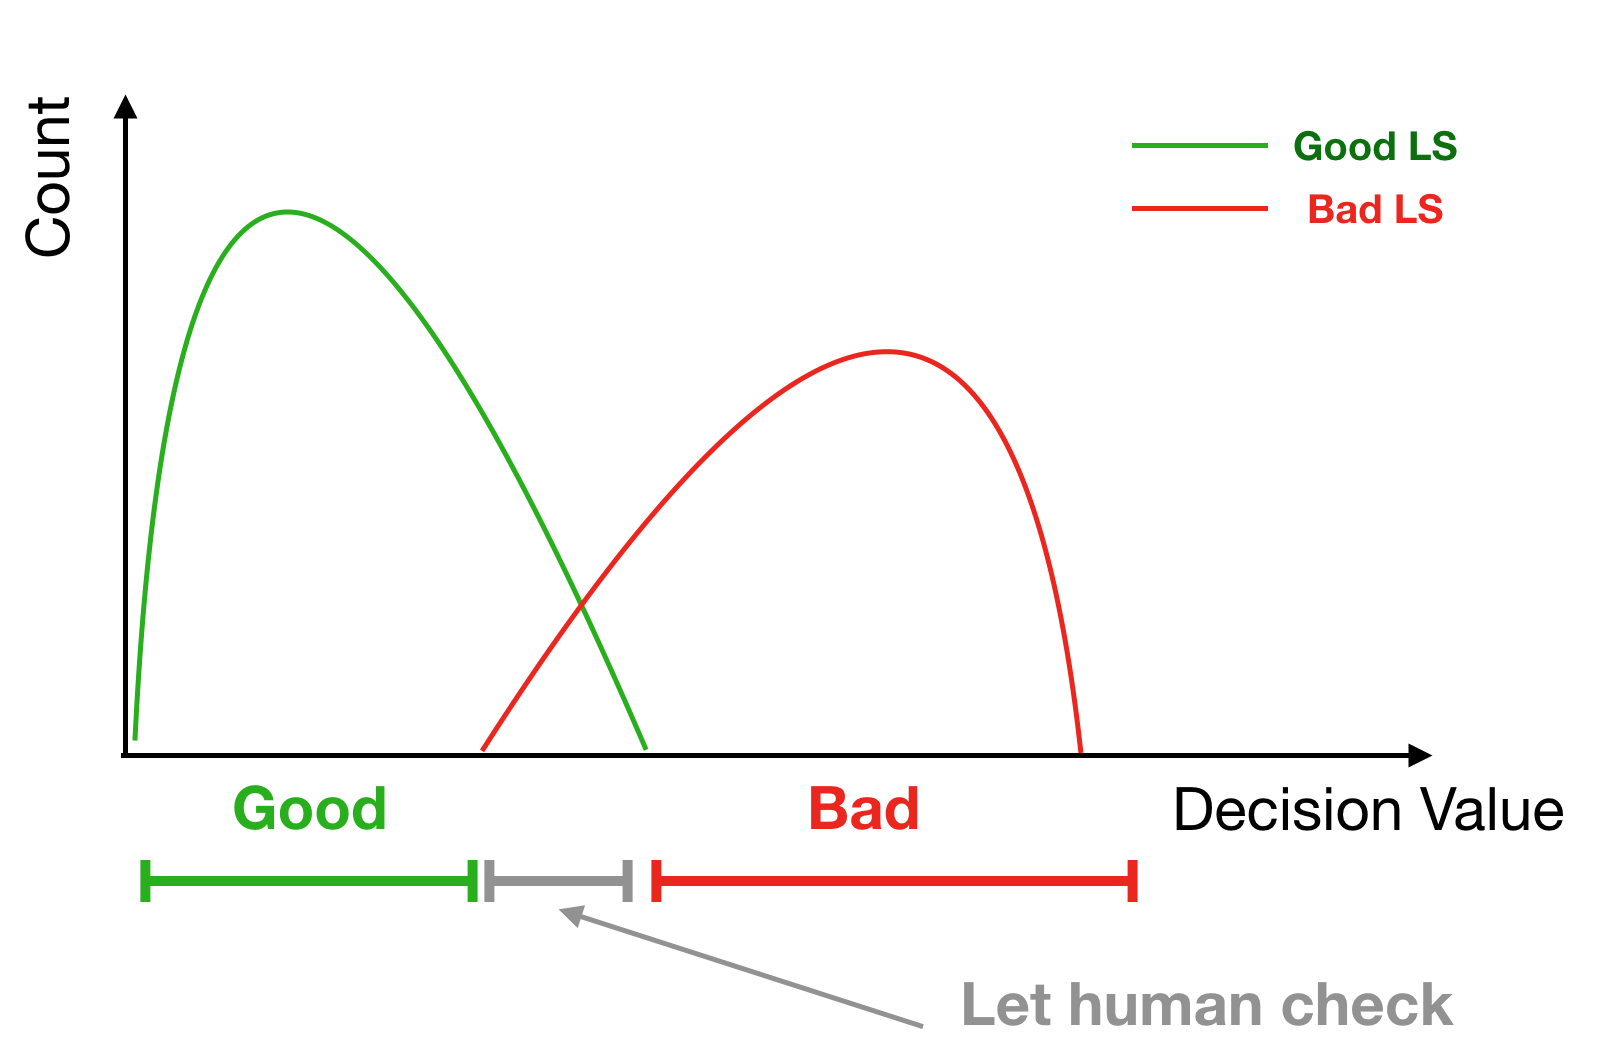
\includegraphics[height=0.7\textheight, width=0.7\textwidth]{images/expected_greyzone}
    \caption{Three possible regions of prediction}
\end{figure}
\end{frame}

%------------------------------------------------
\section{Datasets} % Sections can be created in order to organize your presentation into discrete blocks, all sections and subsections are automatically printed in the table of contents as an overview of the talk
%------------------------------------------------
\subsection{}

%------------------------------------------------
\begin{frame}
\frametitle{Datasets}
\begin{itemize}
    \item pp collisions, 2016 data
    \item JetHT
    \item Each lumisection (datapoint) contains
    \begin{itemize}
        \item 39 histogram of physics quantity e.g. JetPt, JetEta, JetPhi, etc.
        \item Represent one histogram with 7 numbers
        \item 259 Features ( 39 $\times$ 7 )
    \end{itemize}
    \item \textcolor[RGB]{0,128,0}{Good LS} defined in Golden JSON else \textcolor[RGB]{255,0,0}{Bad LS}
    \item Data splitting
    \begin{itemize}
        \item \textcolor[RGB]{0,128,0}{60$\%$} good LSs for training
        \item \textcolor[RGB]{0,128,0}{20$\%$} good LSs for validation
        \item \textcolor[RGB]{128,0,128}{20$\%$} good LSs combine with bad LS for testing
    \end{itemize}
\end{itemize}
\end{frame}
%------------------------------------------------

\begin{frame}
\frametitle{Histogram representation}
\begin{columns}
    \column{0.5\textwidth}
    \begin{figure}
        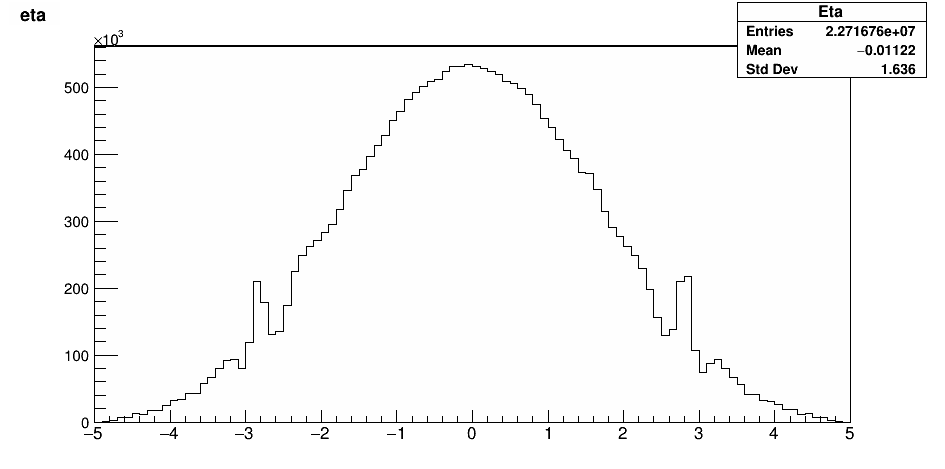
\includegraphics[height=0.4\textheight, width=1.0\textwidth]{images/ex_eta_dist}
        \caption{Example of Eta distribution}
    \end{figure}
    \column{0.5\textwidth}
    \begin{itemize}
    \item Collection of physics objects e.g. photons, muons and so on
    \item Measurement quantity: Transverse momentum, eta, phi, etc.
    \end{itemize}
    \begin{enumerate}
        \item Quantize [10$\%$, 30$\%$, 50$\%$, 70$\%$, 90$\%$] of the histogram
        \item Combine mean and rms
        \item Use these \textbf{7 values to represent one histogram}
    \end{enumerate}
\end{columns}
\end{frame}
    
%------------------------------------------------
\begin{frame}
\frametitle{Data Preprocessing}
\begin{itemize}
    \item MinMaxScalar Transformation
    \item Consider Lumisection $i$ and Feature $j$
    \begin{equation}
        x_{ij}' \leftarrow \frac{x_{ij} - \min_{\forall i\in S_{\text{train}}}\{x_{ij}\}}{\max_{\forall i\in S_{\text{train}}}\{x_{ij}\} - \min_{\forall i\in S_{\text{train}}}\{x_{ij}\} }
    \end{equation}
    \item Then our datapoint should be in range [0, 1]
\end{itemize}
\end{frame}

%------------------------------------------------
\section{Model} % Sections can be created in order to organize your presentation into discrete blocks, all sections and subsections are automatically printed in the table of contents as an overview of the talk
%------------------------------------------------

\begin{frame}
\frametitle{Semi-supervised Learning}
\begin{itemize}
    \item Unsupervised Models
    \begin{itemize}
        \item Sch\"{o}lkopf's One-Class SVM
        \item Isolation Forest
        \item 4 Flavours of Autoencoder
    \end{itemize}
    \item Feed only good LS for train and validate the model
    \item Testing with good LS and bad LS
    \item Consequently, it's falling into \textbf{Semi-supervised Learning} category
\end{itemize}
\end{frame}
    
%------------------------------------------------
\subsection{One-Class SVM}

\begin{frame}
\frametitle{Sch\"{o}lkopf's One-Class SVM}
\begin{columns}
    \column{0.5\textwidth}
    \begin{figure}
        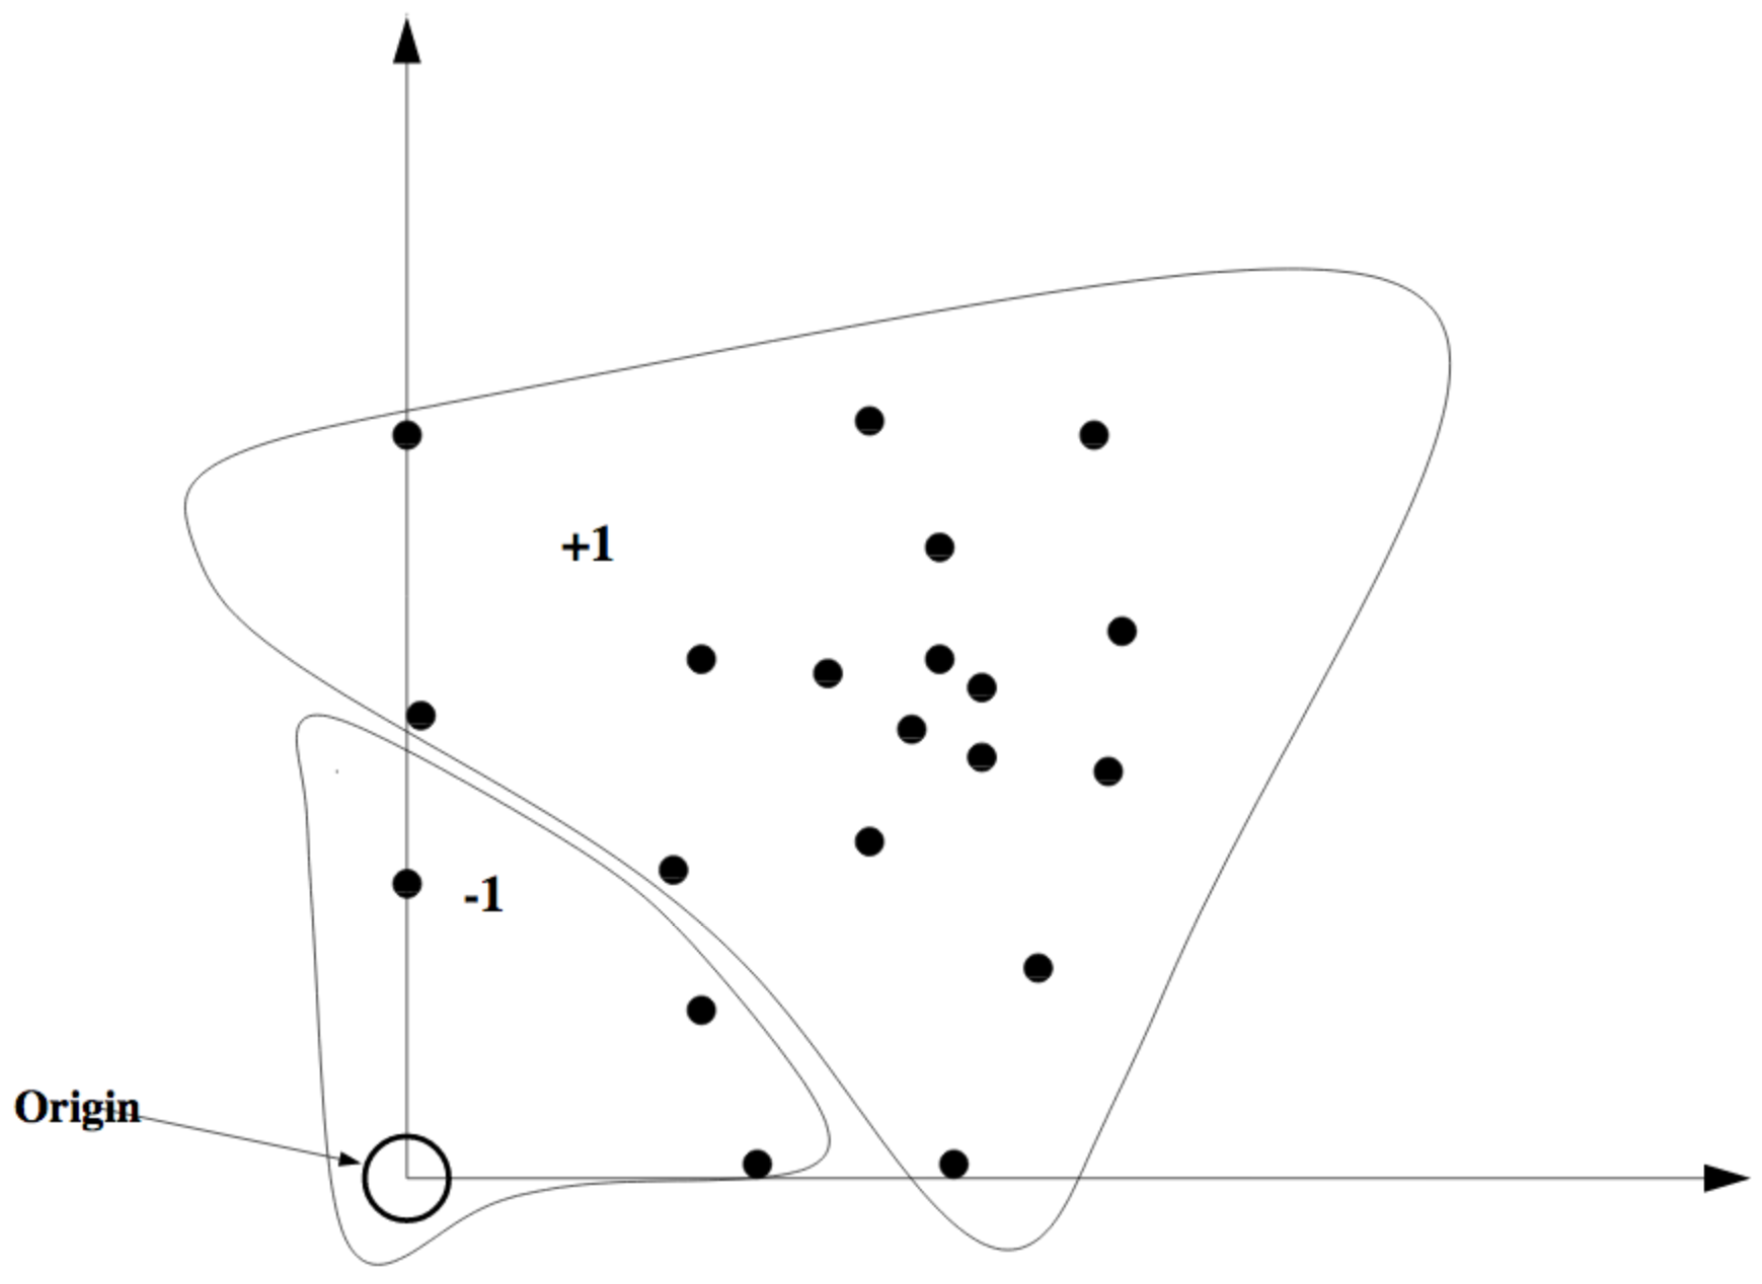
\includegraphics[height=0.5\textheight, width=0.8\textwidth]{images/hyperplane_svm}
        \caption{Scattering in latent space: \tiny retrieved from http://www.jmlr.org/papers/volume2/manevitz01a/manevitz01a.pdf}
    \end{figure}

    \column{0.5\textwidth}
    \begin{itemize}
    \item Minimize (Soft Margin)
    \begin{equation}
        \frac{||w||^2}{2} + \frac{1}{\nu l}\sum_{i=1}^l \xi_i - \rho
    \end{equation}
    \item Under
    \begin{equation}
        w \cdot \Phi(x_i) \geqslant \rho - \xi_i \ ,\ \xi_i \geqslant 0
    \end{equation}
    \item \textbf{Kernel}: Gaussian Base Radial function (GBF)
    \item Determine tangent distance from hyperplane
    \end{itemize}
\end{columns}
\end{frame}

%------------------------------------------------
\subsection{Isolation Forest}

\begin{frame}
\frametitle{Isolation Forest}
\begin{itemize}
    \item Ensemble Forest from tree by subsampling ($\Psi$)
    \begin{itemize}
        \item Iteratively picking up features and random value to construct the node (equivalent to step function)
        \item Anomaly score evaluate from average depth of the instance over forest
        \begin{equation}
            s(x, \Psi) = \exp^{-<h(x)>/c(\Psi)}
        \end{equation}
        \item where
        \begin{itemize}
            \item $h(x)$ is the depth in tree $h$
            \item $c(\Psi)$ normalization factor growing as $\log_2(\Psi)$ from branching
        \end{itemize}
    \end{itemize}
\end{itemize}
\vspace{0.2in} \tiny [1] https://cs.nju.edu.cn/zhouzh/zhouzh.files/publication/icdm08b.pdf?q=isolation-forest
\end{frame}

%------------------------------------------------
\subsection{Autoencoder}

\begin{frame}
\frametitle{Vanilla Autoencoder}
\begin{columns}
    \column{0.5\textwidth}
    \begin{figure}
        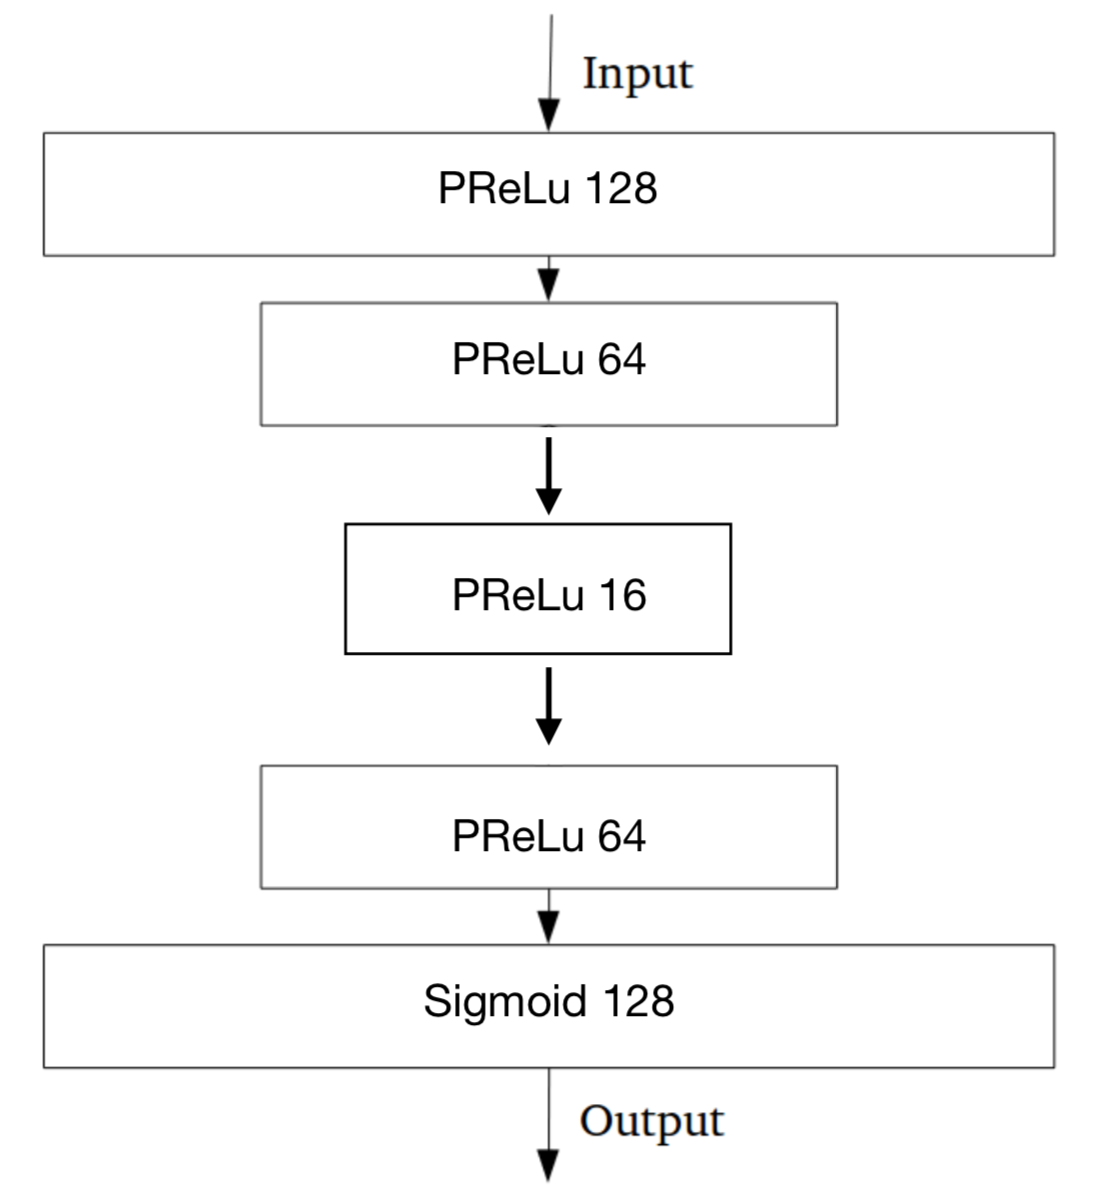
\includegraphics[height=0.6\textheight, width=0.7\textwidth]{images/vanilla_ae}
        \caption{Body of Vanilla AE}
    \end{figure}

    \column{0.5\textwidth}
    \begin{itemize}
    \item Concise the information into small latent space and reconstruct
    \item Loss function
    \begin{equation}
        \mathcal{L}_{\text{tot}} \equiv \frac{1}{N}\sum_i^N |x-\tilde{x}|^2
    \end{equation}
    \item Truncated normal initializer
    \item Adam optimizer
    \end{itemize}
\end{columns}
\end{frame}
%------------------------------------------------
\begin{frame}
\frametitle{Sparse Autoencoder}
\begin{itemize}
    \item Similar to Vanilla AE
    \item Tweak by \textcolor[RGB]{255,69,0}{L1 Regularizaion (Prevent overfitting)}
    \item Loss function
    \begin{equation}
        \mathcal{L}_{\text{tot}} \equiv \frac{1}{N}\sum_i^N |x-\tilde{x}|^2 + \textcolor[RGB]{255,69,0}{\lambda_{\text{s}}\sum_j||w_j||}
    \end{equation}
    \item where $\lambda_{\text{s}} = 10^{-5}$
\end{itemize}

\end{frame}
%------------------------------------------------
\begin{frame}
\frametitle{Contractive Autoencoder}

\begin{itemize}
    \item Tweak by \textcolor[RGB]{0,128,0}{Jacobi Matrix (Prevent variation in dataset)}
    \item Loss function
    \begin{equation}
        \mathcal{L}_{\text{tot}} \equiv \frac{1}{N}\sum_i^N |x-\tilde{x}|^2 + \textcolor[RGB]{0,128,0}{\lambda_{\text{c}}||J_h(x)||^2}
    \end{equation}
    \item where $\lambda_{\text{c}} = 10^{-5}$
\end{itemize}
\end{frame}
%------------------------------------------------
\begin{frame}
\frametitle{Contractive Autoencoder}
\begin{itemize}
    \item Definition
    \begin{equation}
        \textcolor[RGB]{0,128,0}{||J_h(x)||^2 \equiv \sum_{ij}\left(\frac{\partial h_j}{\partial x_i}\right)^2}
    \end{equation}
    \item where $h_j$ is activation function
    \item In our cases
    \begin{itemize}
        \item PReLu activation function
        \begin{equation}
            ||J_h(x)||^2 = \sum_j[\alpha_jH(-(w_{ji}x^i+b_j)) + H(w_{ji}x^i+b_j)]\sum_i(w_{ji})^2
        \end{equation}
        \item Sigmoid activation function
        \begin{equation}
            ||J_h(x)||^2 = \sum_j[h_j*(1-h_j)]\sum_i(w_{ji})^2
        \end{equation}
    \end{itemize}
\end{itemize}

\end{frame}

%------------------------------------------------
\begin{frame}
\frametitle{Variational Autoencoder}
\begin{columns}
    \column{0.5\textwidth}
    \begin{figure}
        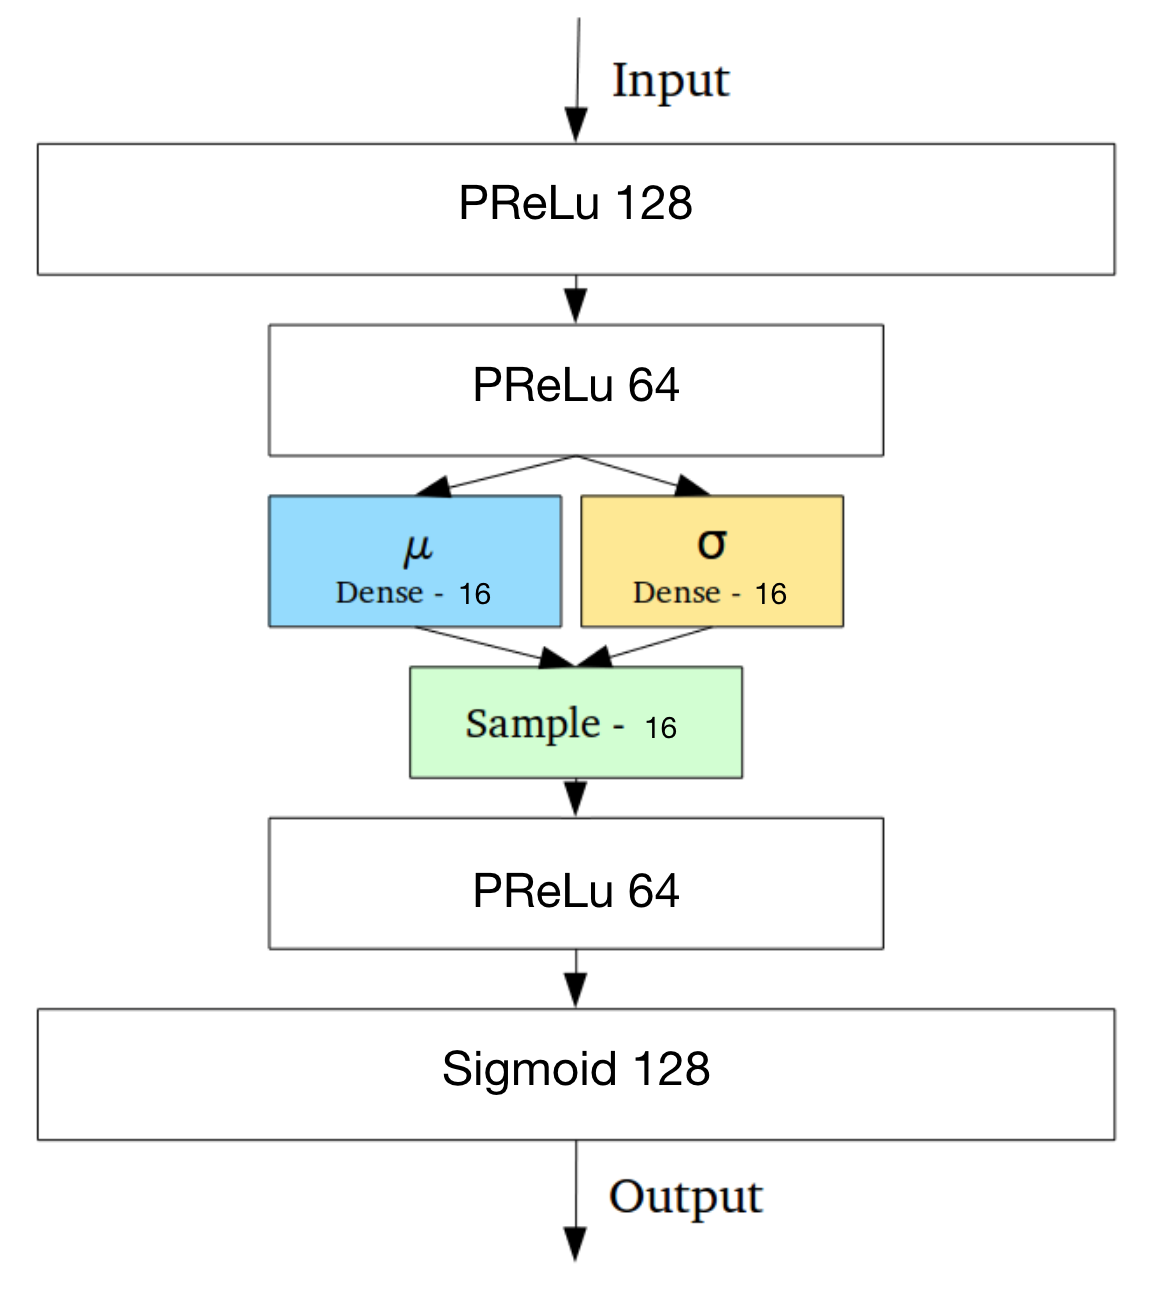
\includegraphics[height=0.6\textheight, width=0.6\textwidth]{images/variational_ae}
        \caption{Body of Variational AE \tiny retrieved from https://towardsdatascience.com/intuitively-understanding-variational-autoencoders-1bfe67eb5daf}
    \end{figure}

    \column{0.5\textwidth}
    \begin{itemize}
        \item Random \say{new sampling} in latent space by gaussian random generator
        \begin{equation}
            \mathcal{Z} \equiv \mathcal{N}(\mu_i, \sigma_i)
        \end{equation}
        \item Tweak by \textcolor[RGB]{148,0,211}{reduce discontinuity in latent space}
        \item Loss function
        \begin{equation}
            \mathcal{L}_{\text{tot}} = \frac{1}{N}\sum_i^N |x-\tilde{x}|^2 + \textcolor[RGB]{148,0,211}{\mathcal{D}_{\text{KL}}(p|q)}
        \end{equation}
    \end{itemize}
\end{columns}
\end{frame}
%------------------------------------------------
\begin{frame}
\frametitle{Variational Autoencoder}
\begin{theorem}[Kullback-Leibler Divergence]
\begin{itemize}
    \item \say{How much information is loss after represent data with function}
    \begin{equation}
        \mathcal{D}_{\text{KL}} \equiv < \log p - \log q >
    \end{equation}
    \item Where $p$ is observed value and $q$ is approximaiton function
    \item Since our $q$ is Gaussian function
    \begin{equation}
        \mathcal{D}_{\text{KL}} = \frac{1}{2}(\mu_i^2 +\sigma_i^2 - 2\log(\sigma_i) - 1)
    \end{equation}
\end{itemize}
\end{theorem}
\begin{equation}
    \mathcal{L}_{\text{tot}} = \frac{1}{N}\sum_i^N |x-\tilde{x}|^2 + \textcolor[RGB]{148,0,211}{\frac{1}{2}(\mu_i^2 +\sigma_i^2 - 2\log(\sigma_i) - 1)}
\end{equation}
\end{frame}

%------------------------------------------------
\section{Results and Interpretation}
%------------------------------------------------
\subsection{}

\begin{frame}
\frametitle{Find the cutoff}
\begin{figure}
    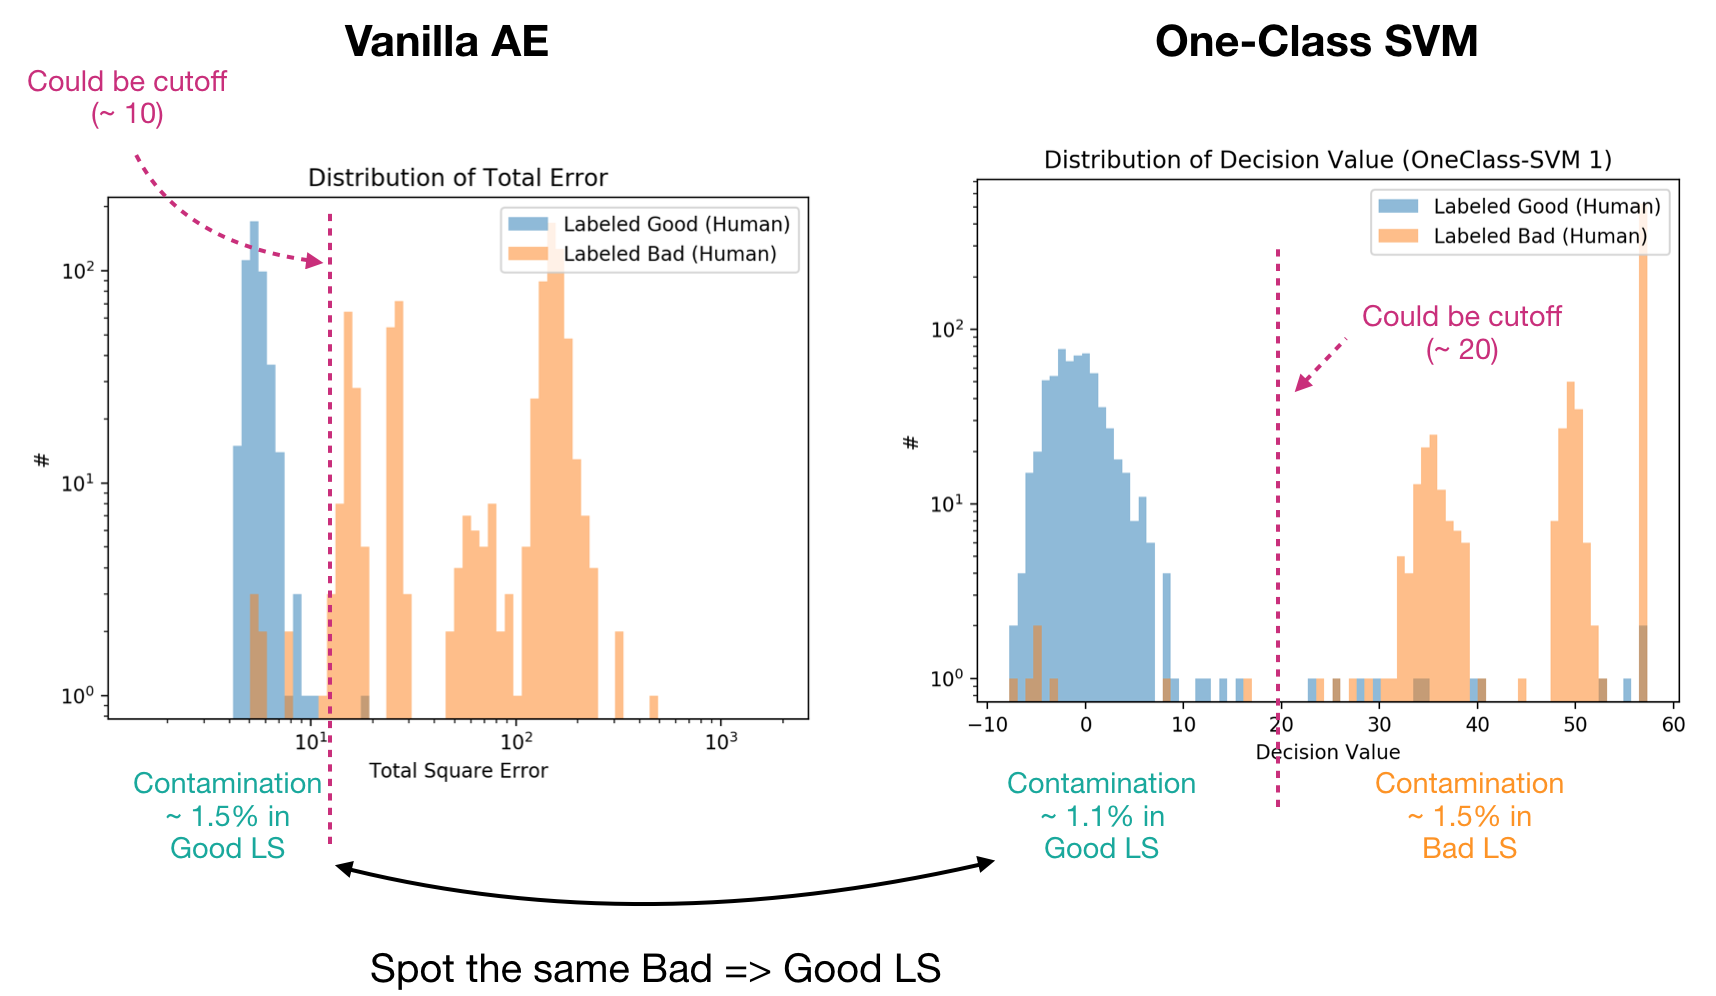
\includegraphics[height=0.8\textheight, width=0.95\textwidth]{images/decision_value_dist}
\end{figure}
\end{frame}

%------------------------------------------------
\begin{frame}
\frametitle{Performance}
\begin{columns}
    \column{0.5\textwidth}
    \begin{figure}
        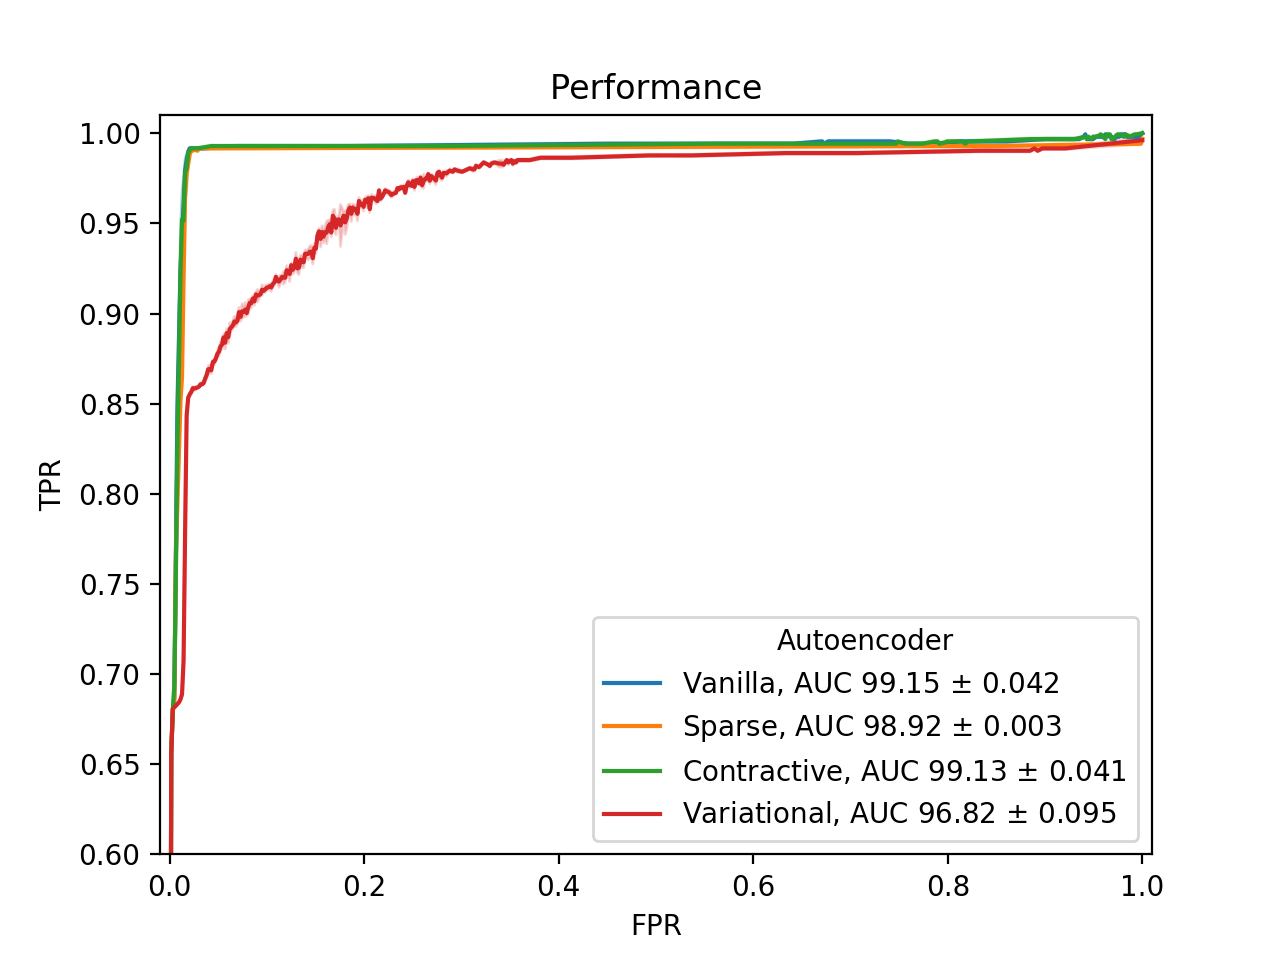
\includegraphics[height=0.55\textheight, width=0.95\textwidth]{images/performance_ae}
        \caption{Various AE}
    \end{figure}
    \column{0.5\textwidth}
    \begin{figure}
        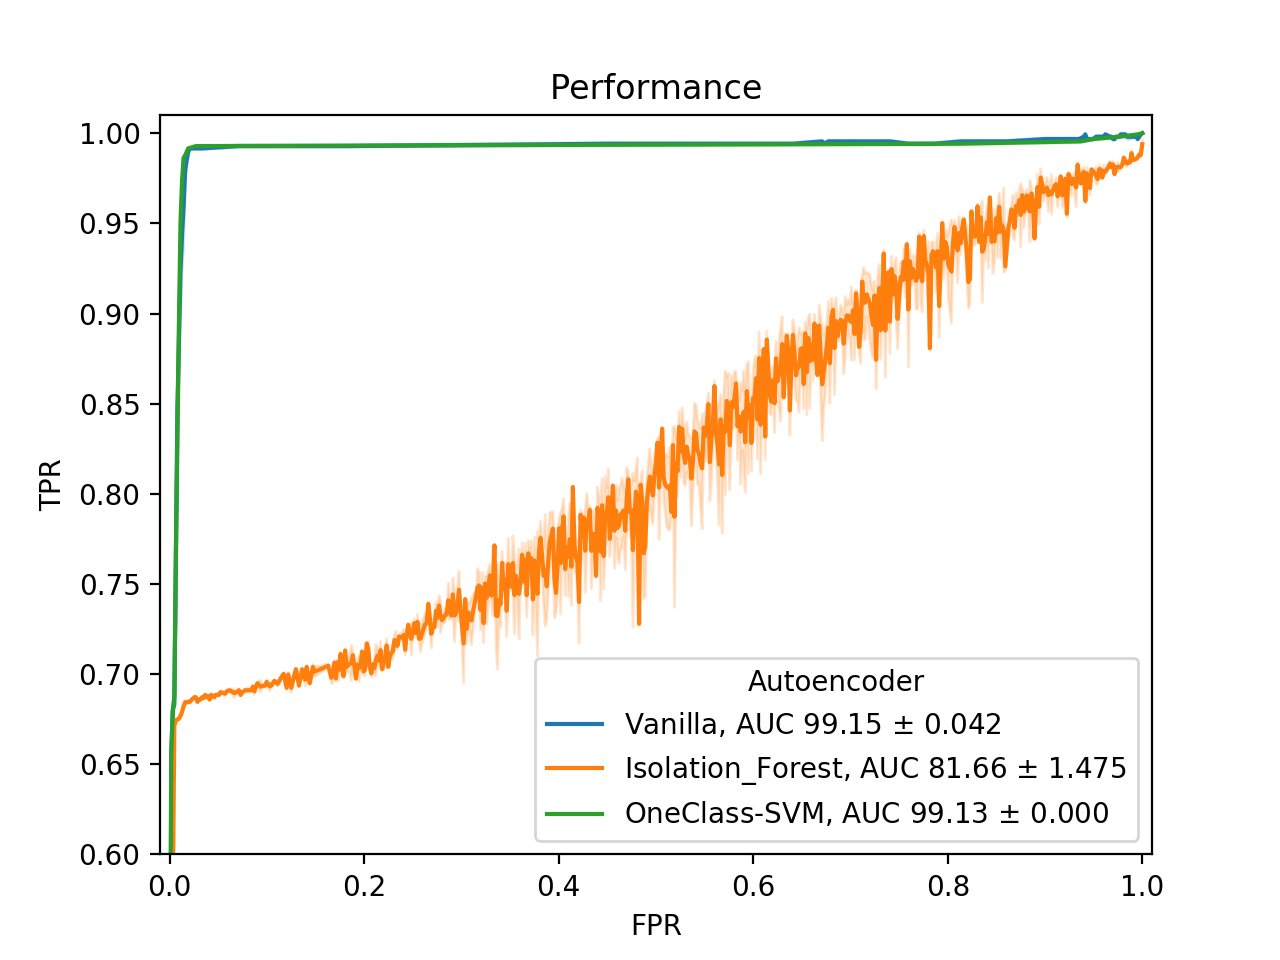
\includegraphics[height=0.55\textheight, width=0.95\textwidth]{images/performance_ml}
        \caption{Vanilla vs SVM vs Forest}
    \end{figure}
\end{columns}
\tiny
Under configuration
\begin{itemize}
    \item \textbf{Isolation Forest}  $N_{\text{tree}} = 200,\ \Psi = 512$
    \item \textbf{OneClass-SVM} $\nu = 0.1,\ \gamma = 0.1$(Inverse gaussian width)
\end{itemize}
\end{frame}

%------------------------------------------------
\begin{frame}
\frametitle{Example of Reconstruction}
\begin{figure}
    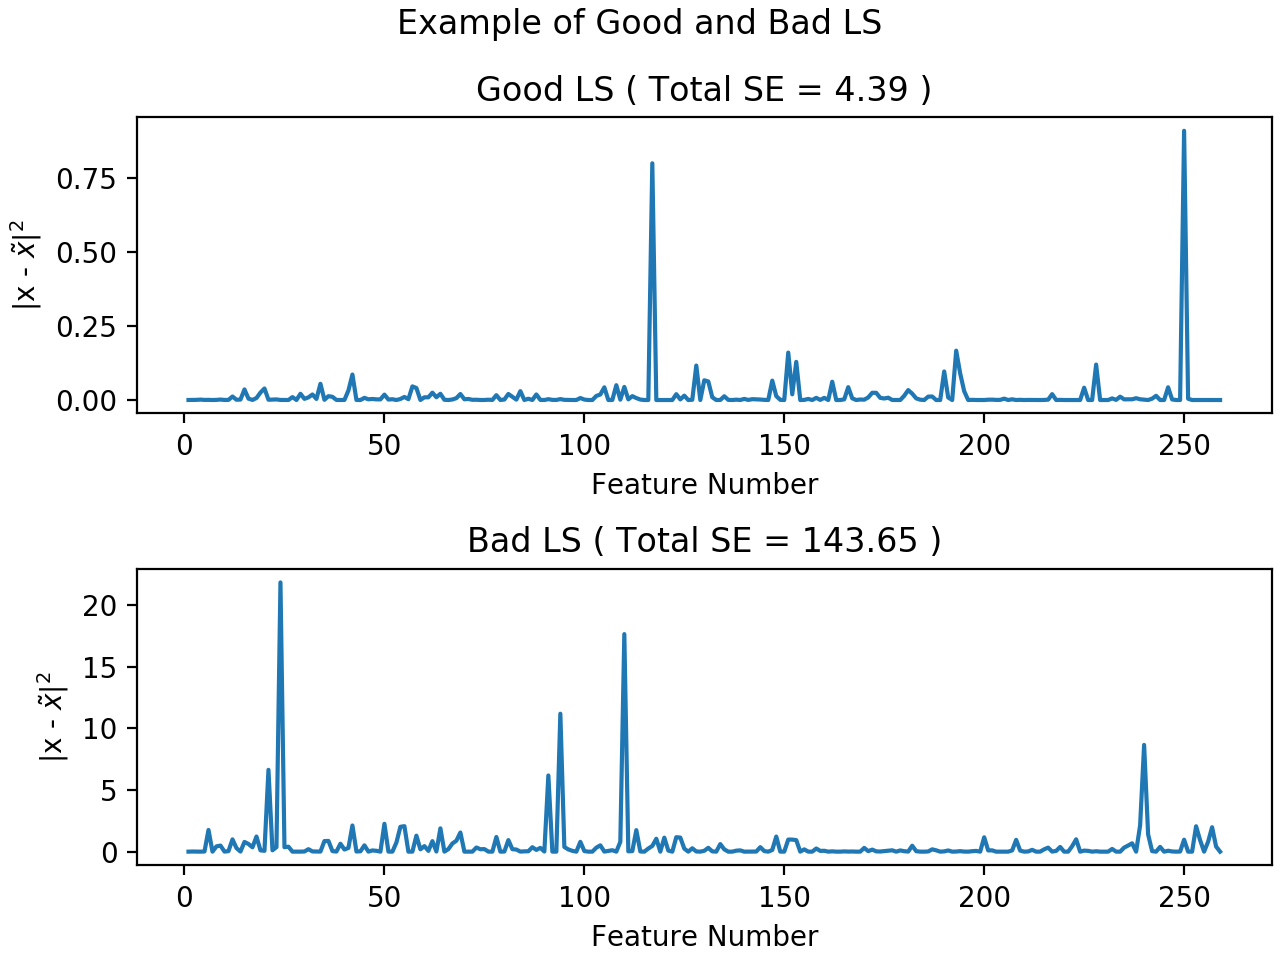
\includegraphics[height=0.7\textheight, width=0.7\textwidth]{images/example_se}
    \caption{Reconstruction error from Vanilla AE}
\end{figure}
\end{frame}

%------------------------------------------------
\begin{frame}
\frametitle{Extended Investigation}
\begin{figure}
    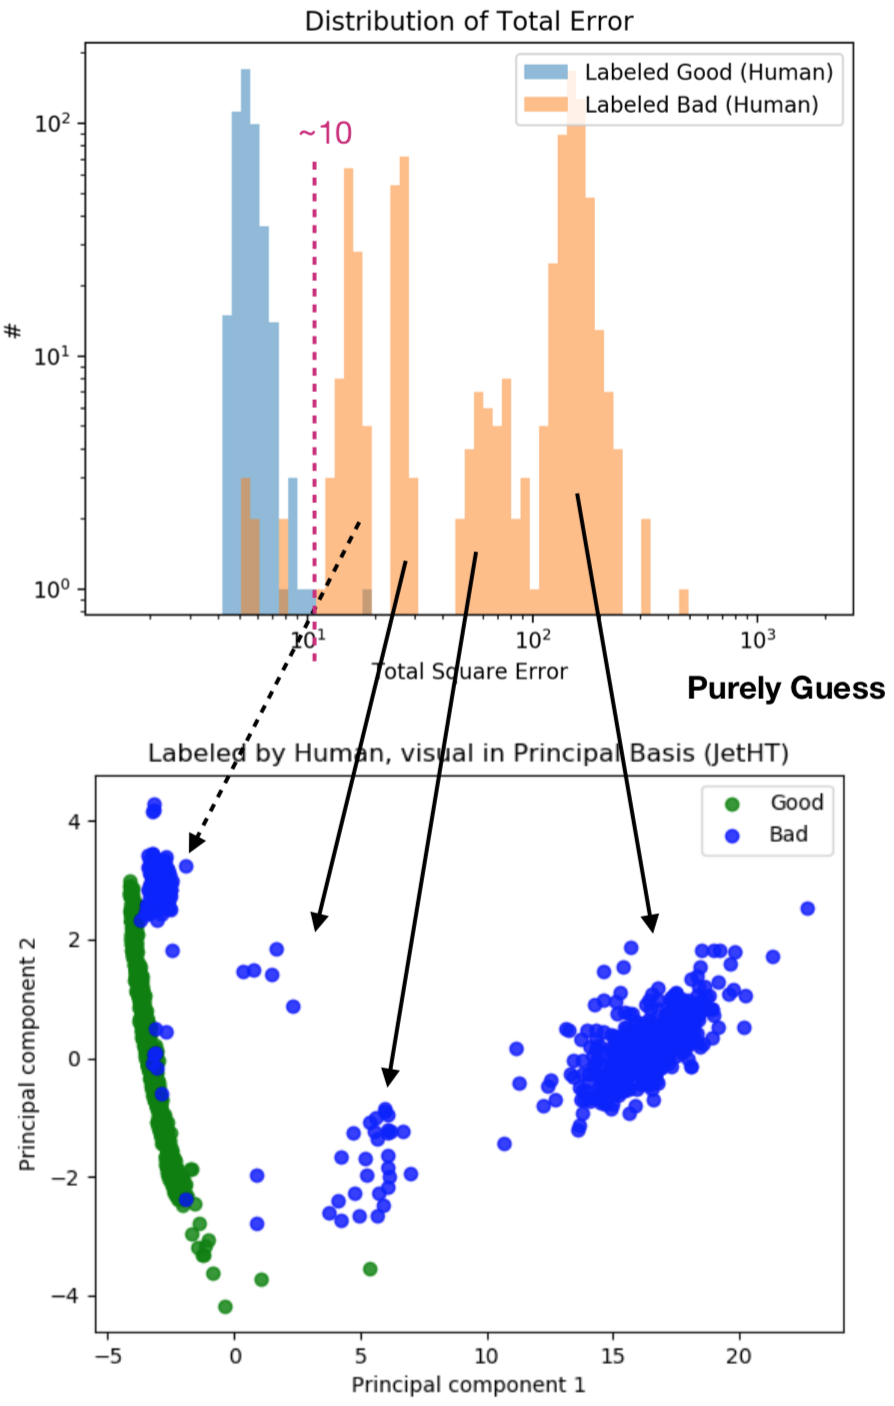
\includegraphics[height=0.85\textheight, width=0.4\textwidth]{images/guess}
\end{figure}
\end{frame}

%------------------------------------------------
\begin{frame}
\frametitle{Extended Investigation}
\begin{figure}
    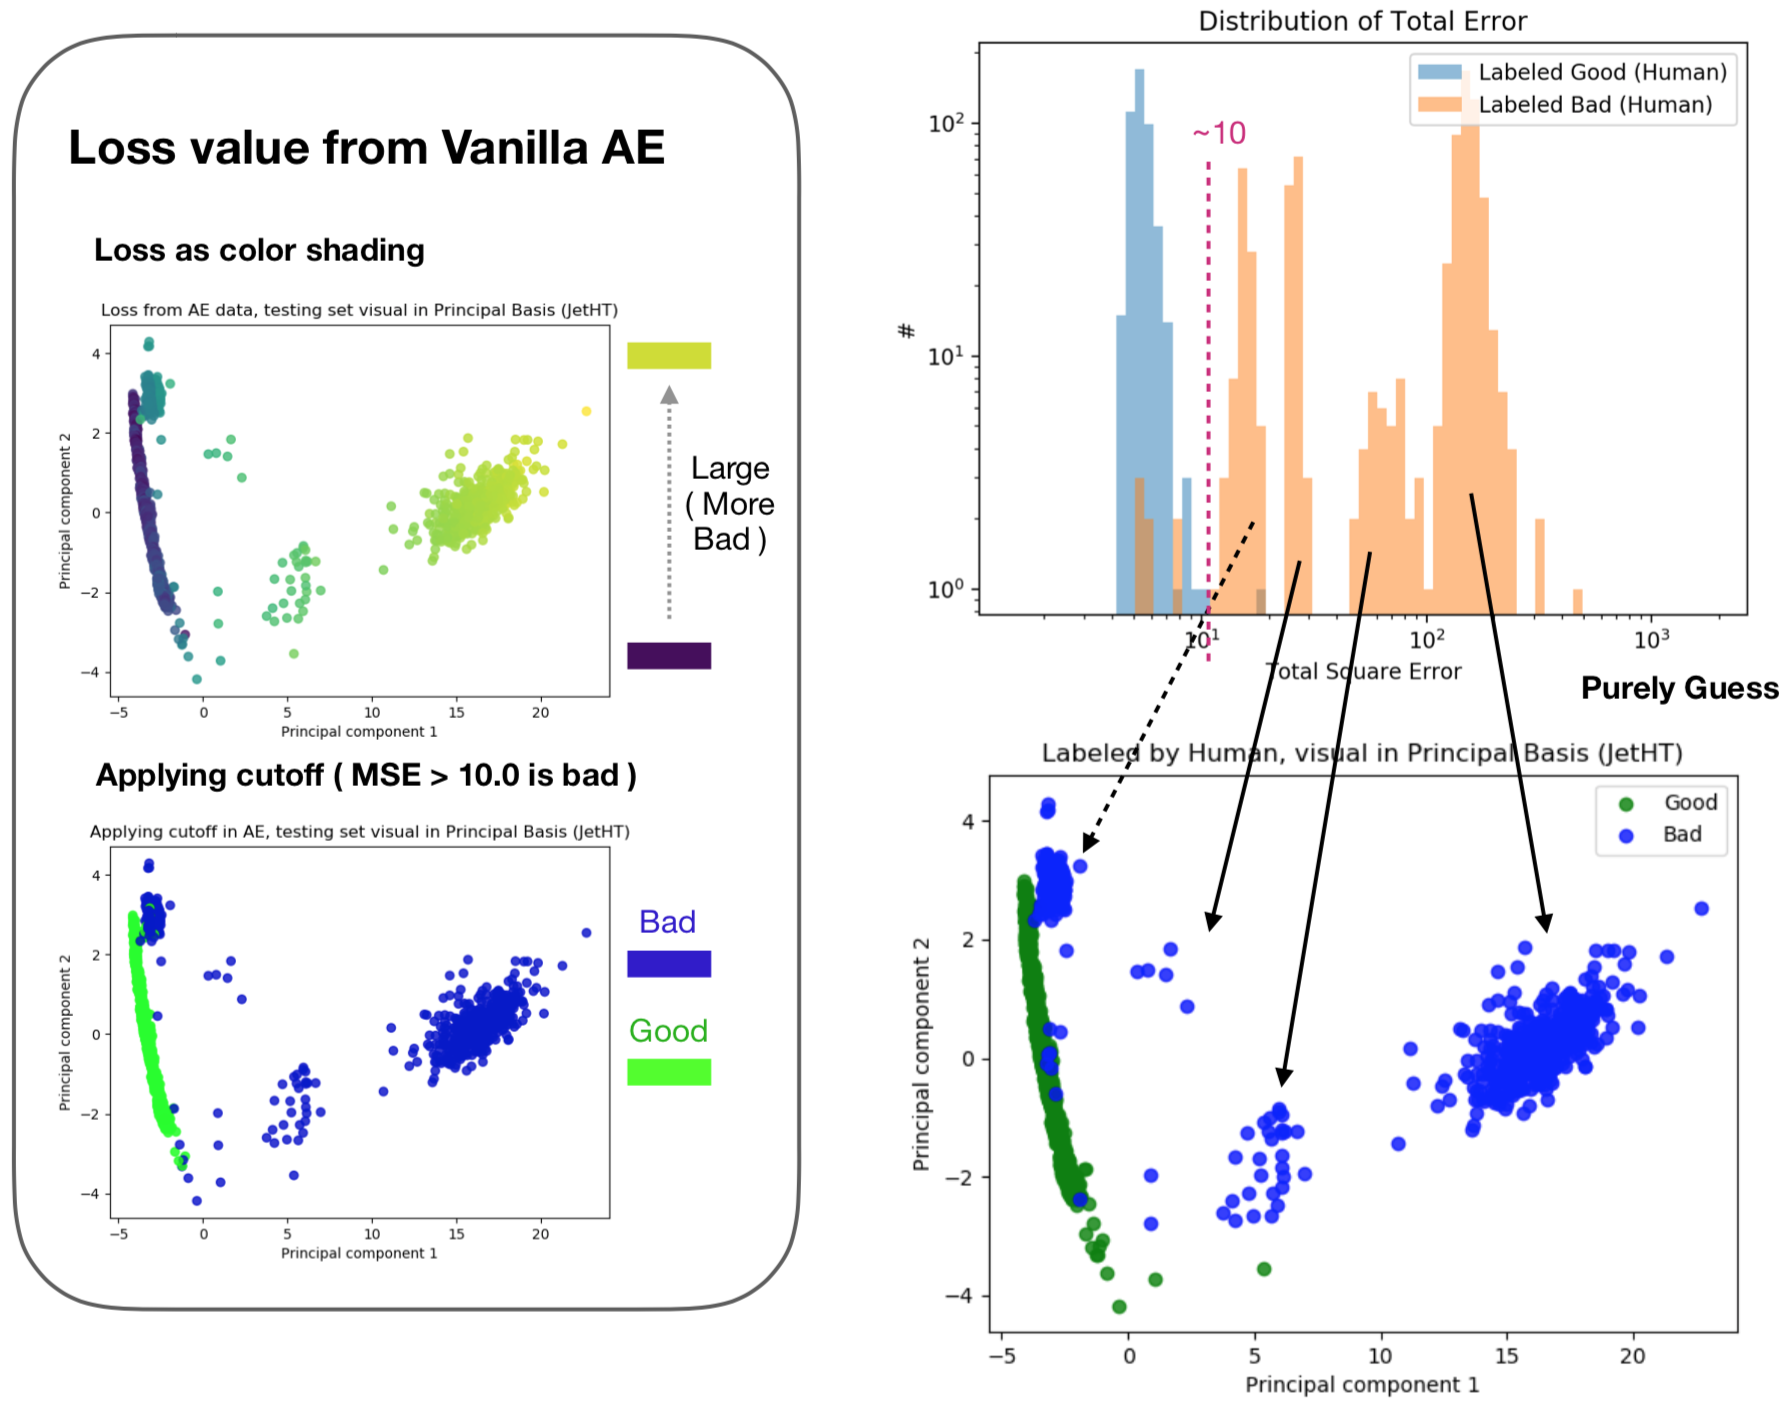
\includegraphics[height=0.85\textheight, width=0.75\textwidth]{images/guess_visual}
\end{figure}
\end{frame}

%------------------------------------------------
\section{Summary} % Sections can be created in order to organize your presentation into discrete blocks, all sections and subsections are automatically printed in the table of contents as an overview of the talk
%------------------------------------------------
\begin{frame}
\frametitle{Summary}
\begin{itemize}
    \item Semi-supervised learning yield a remarkable result
    \item There is no grey zone from our model for this dataset
    \item Bad LS could be divided into two parts
    \begin{itemize}
        \item Bad with some pattern
        \item Anomaly
    \end{itemize}
\end{itemize}
\begin{figure}
    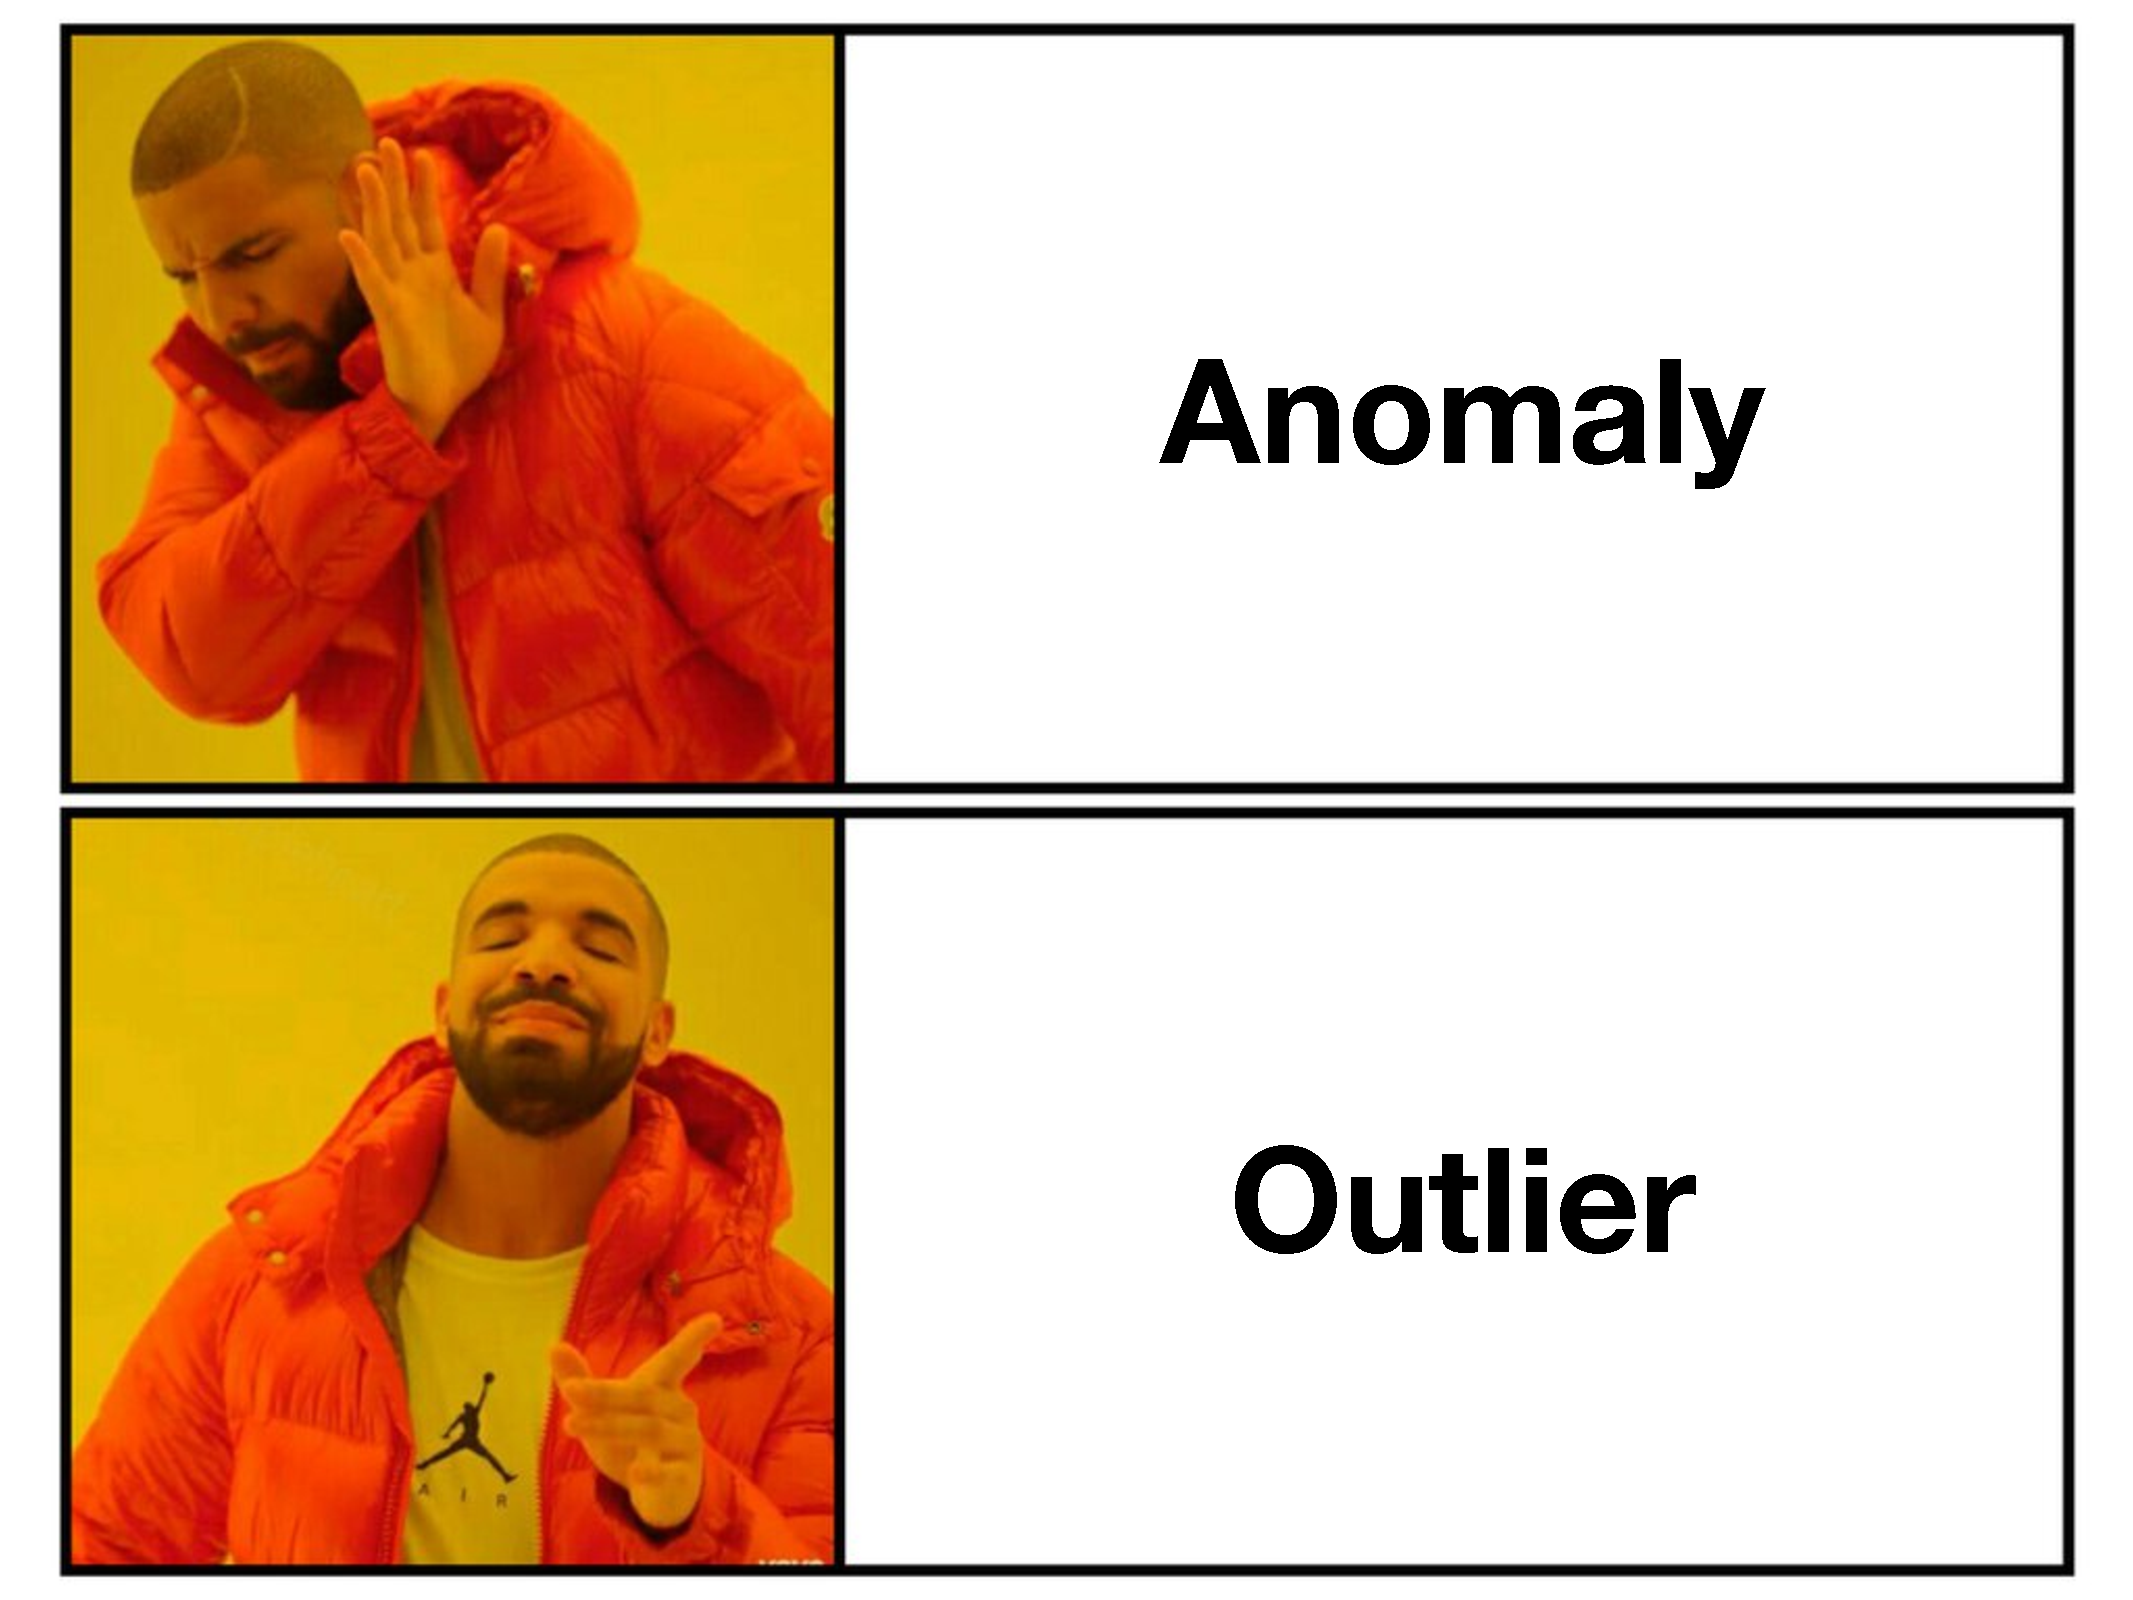
\includegraphics[height=0.4\textheight, width=0.35\textwidth]{images/meme_outlier}
\end{figure}
\end{frame}
%------------------------------------------------
\begin{frame}
\frametitle{Future work}
\begin{itemize}
    \item Good LS from run tagged by human and DCS bits still suspicious not to be a ground truth
    \item Require simulation data
    \begin{itemize}
        \item To be purely good LS for training
        \item For testing the failure scenario
    \end{itemize}
\end{itemize}
\end{frame}

%------------------------------------------------
\section{}
\begin{frame}
\frametitle{Acknowledgement}
\begin{itemize}
    \item CERN Summer Student program 2019
    \item Especially
    \begin{itemize}
        \item Marcel Andre Schneider
        \item Francesco Fiori
        \item Kaori Maeshima
        \item also countless DQM people :)
    \end{itemize}
    \item GPU Resources from IBM
\end{itemize}
\end{frame}

\begin{frame}
\Huge{\centerline{Thank you}}
\end{frame}
\begin{frame}
\Huge{\centerline{Question?}}
\end{frame}

%------------------------------------------------
%   Back up slide
%------------------------------------------------
\begin{frame}
\Huge{\centerline{Back up}}
\end{frame}

%------------------------------------------------
\begin{frame}
\frametitle{ROC Curve}
bla
\end{frame}

%----------------------------------------------------------------------------------------
\end{document} 